\documentclass[11pt,letterpaper]{article}
\usepackage[top=0.7in,bottom=0.6in,left=0.7in,right=0.7in]{geometry}
\usepackage{fontspec}\usepackage{graphicx}\graphicspath{{../../../../papers/notepat-charts/}}\usepackage{xcolor}\usepackage{amsmath}
\setmainfont[Extension=.otf,UprightFont=lmroman10-regular,BoldFont=lmroman10-bold,ItalicFont=lmroman10-italic]{lmroman10}
\setsansfont[Extension=.otf,UprightFont=lmsans10-regular,BoldFont=lmsans10-bold]{lmsans10}
\setmonofont[Extension=.otf,UprightFont=lmmono10-regular]{lmmono10}
\definecolor{cream}{HTML}{F6F0E2}\definecolor{ink}{HTML}{1E1A14}\definecolor{red}{HTML}{C03A2B}\definecolor{blue}{HTML}{2457A8}
\pagecolor{cream}\color{ink}\pagestyle{empty}
\newcommand{\chord}[1]{\sffamily\bfseries\color{red}\large #1}
\newcommand{\rh}[1]{\ttfamily\fontsize{30}{34}\selectfont\color{ink}#1}
\newcommand{\lh}[1]{\ttfamily\fontsize{17}{20}\selectfont\color{blue}#1}
\begin{document}
\begin{center}{\fontsize{40}{44}\selectfont\bfseries QWERTY Waltzes}\\[6pt]{\large three waltzes for one notepat keyboard, left hand and right}\\[4pt]{\small by @jeffrey with Claude · aesthetic.computer · November 2026}\\[18pt]
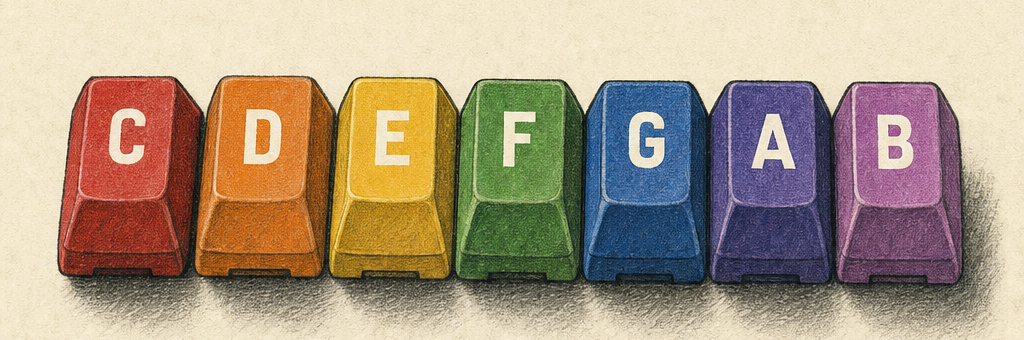
\includegraphics[width=0.9\textwidth]{keys-strip.png}\\[18pt]\end{center}
{\large\noindent\textbf{How to read a card.} Each box is one bar of three beats. The red word is the chord. The big letters are the right hand: one key per beat, and a dash means keep holding the last key. The blue line is the left hand: press the single key on beat one, then press the two keys together on beats two and three. Letters are notepat letters: \texttt{c d e f g a b} are the low octave, \texttt{h i j k l m n} the high one, and the sharps sit one row up (\texttt{r} is G$\sharp$, \texttt{w} is F$\sharp$ low, \texttt{u} is F$\sharp$ high, \texttt{o} is G$\sharp$ high). Count ``ONE two three'' and let the left hand do the waltz; the right hand only ever moves to a neighbour or a chord tone.}\par\vspace{14pt}
{\large\noindent\textbf{Learning order.} Left hand alone until the bass-chord-chord rocks without looking. Then right hand alone, singing the letters. Then together at half speed. Menu Band plays each score when you open its \texttt{.mbscore}; play along with the file, then without it.}
\clearpage

\begin{center}
{\fontsize{34}{38}\selectfont\bfseries Home Row Waltz}\\[4pt]
{\large C major \quad·\quad $\frac{3}{4}$ \quad·\quad 132 bpm \quad·\quad 16 bars}\\[6pt]
{\small\itshape right hand lives on h i j k l m n; left hand rocks c, f, g with e+g, f+a, b+d}\\[10pt]
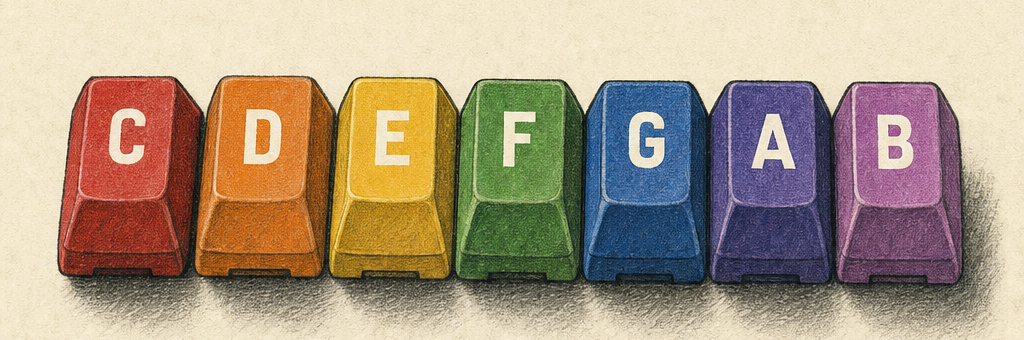
\includegraphics[width=0.62\textwidth]{keys-strip.png}\\[14pt]
\end{center}
{\small\sffamily top line = chord · middle = right hand, one letter per beat, – holds the note · bottom = left hand: bass on 1, then the two-key chord on 2 and 3}\par\vspace{16pt}
\noindent\begin{minipage}[t]{0.23\textwidth}\centering{\chord C}\\[2pt]{\rh h j l}\\[2pt]{\lh c\ \ e+g\ \ e+g}\end{minipage}\hfill\begin{minipage}[t]{0.23\textwidth}\centering{\chord C}\\[2pt]{\rh l – –}\\[2pt]{\lh c\ \ e+g\ \ e+g}\end{minipage}\hfill\begin{minipage}[t]{0.23\textwidth}\centering{\chord F}\\[2pt]{\rh k m k}\\[2pt]{\lh f\ \ f+a\ \ f+a}\end{minipage}\hfill\begin{minipage}[t]{0.23\textwidth}\centering{\chord C}\\[2pt]{\rh j – –}\\[2pt]{\lh c\ \ e+g\ \ e+g}\end{minipage}\par\vspace{14pt}\vspace{2pt}\noindent\begin{minipage}[t]{0.23\textwidth}\centering{\chord G}\\[2pt]{\rh i k i}\\[2pt]{\lh g\ \ b+d\ \ b+d}\end{minipage}\hfill\begin{minipage}[t]{0.23\textwidth}\centering{\chord G}\\[2pt]{\rh n – –}\\[2pt]{\lh g\ \ b+d\ \ b+d}\end{minipage}\hfill\begin{minipage}[t]{0.23\textwidth}\centering{\chord C}\\[2pt]{\rh h j l}\\[2pt]{\lh c\ \ e+g\ \ e+g}\end{minipage}\hfill\begin{minipage}[t]{0.23\textwidth}\centering{\chord G}\\[2pt]{\rh i – –}\\[2pt]{\lh g\ \ b+d\ \ b+d}\end{minipage}\par\vspace{14pt}\noindent\rule{\textwidth}{0.4pt}\par\vspace{12pt}\noindent\begin{minipage}[t]{0.23\textwidth}\centering{\chord C}\\[2pt]{\rh l l m}\\[2pt]{\lh c\ \ e+g\ \ e+g}\end{minipage}\hfill\begin{minipage}[t]{0.23\textwidth}\centering{\chord C}\\[2pt]{\rh l j h}\\[2pt]{\lh c\ \ e+g\ \ e+g}\end{minipage}\hfill\begin{minipage}[t]{0.23\textwidth}\centering{\chord F}\\[2pt]{\rh k k m}\\[2pt]{\lh f\ \ f+a\ \ f+a}\end{minipage}\hfill\begin{minipage}[t]{0.23\textwidth}\centering{\chord F}\\[2pt]{\rh k – –}\\[2pt]{\lh f\ \ f+a\ \ f+a}\end{minipage}\par\vspace{14pt}\vspace{2pt}\noindent\begin{minipage}[t]{0.23\textwidth}\centering{\chord G}\\[2pt]{\rh i j k}\\[2pt]{\lh g\ \ b+d\ \ b+d}\end{minipage}\hfill\begin{minipage}[t]{0.23\textwidth}\centering{\chord G}\\[2pt]{\rh l – –}\\[2pt]{\lh g\ \ b+d\ \ b+d}\end{minipage}\hfill\begin{minipage}[t]{0.23\textwidth}\centering{\chord G}\\[2pt]{\rh i j i}\\[2pt]{\lh g\ \ b+d\ \ b+d}\end{minipage}\hfill\begin{minipage}[t]{0.23\textwidth}\centering{\chord C}\\[2pt]{\rh h – –}\\[2pt]{\lh c\ \ e+g\ \ e+g}\end{minipage}\par\vspace{14pt}\vspace{2pt}
\clearpage
\begin{center}
{\fontsize{34}{38}\selectfont\bfseries Minor Waltz}\\[4pt]
{\large A minor \quad·\quad $\frac{3}{4}$ \quad·\quad 112 bpm \quad·\quad 16 bars}\\[6pt]
{\small\itshape one sharp in the left hand: r is G$\sharp$. the E chord is e with r+b}\\[10pt]
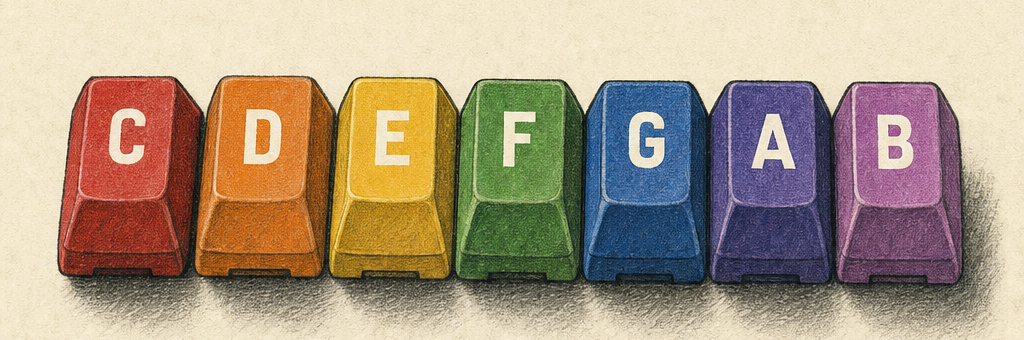
\includegraphics[width=0.62\textwidth]{keys-strip.png}\\[14pt]
\end{center}
{\small\sffamily top line = chord · middle = right hand, one letter per beat, – holds the note · bottom = left hand: bass on 1, then the two-key chord on 2 and 3}\par\vspace{16pt}
\noindent\begin{minipage}[t]{0.23\textwidth}\centering{\chord Am}\\[2pt]{\rh j m j}\\[2pt]{\lh a\ \ c+e\ \ c+e}\end{minipage}\hfill\begin{minipage}[t]{0.23\textwidth}\centering{\chord Am}\\[2pt]{\rh h – –}\\[2pt]{\lh a\ \ c+e\ \ c+e}\end{minipage}\hfill\begin{minipage}[t]{0.23\textwidth}\centering{\chord Dm}\\[2pt]{\rh i k i}\\[2pt]{\lh d\ \ f+a\ \ f+a}\end{minipage}\hfill\begin{minipage}[t]{0.23\textwidth}\centering{\chord Am}\\[2pt]{\rh j – –}\\[2pt]{\lh a\ \ c+e\ \ c+e}\end{minipage}\par\vspace{14pt}\vspace{2pt}\noindent\begin{minipage}[t]{0.23\textwidth}\centering{\chord E}\\[2pt]{\rh o n o}\\[2pt]{\lh e\ \ r+b\ \ r+b}\end{minipage}\hfill\begin{minipage}[t]{0.23\textwidth}\centering{\chord E}\\[2pt]{\rh j – –}\\[2pt]{\lh e\ \ r+b\ \ r+b}\end{minipage}\hfill\begin{minipage}[t]{0.23\textwidth}\centering{\chord Am}\\[2pt]{\rh h i j}\\[2pt]{\lh a\ \ c+e\ \ c+e}\end{minipage}\hfill\begin{minipage}[t]{0.23\textwidth}\centering{\chord E}\\[2pt]{\rh n – –}\\[2pt]{\lh e\ \ r+b\ \ r+b}\end{minipage}\par\vspace{14pt}\noindent\rule{\textwidth}{0.4pt}\par\vspace{12pt}\noindent\begin{minipage}[t]{0.23\textwidth}\centering{\chord Am}\\[2pt]{\rh m – l}\\[2pt]{\lh a\ \ c+e\ \ c+e}\end{minipage}\hfill\begin{minipage}[t]{0.23\textwidth}\centering{\chord Am}\\[2pt]{\rh k – j}\\[2pt]{\lh a\ \ c+e\ \ c+e}\end{minipage}\hfill\begin{minipage}[t]{0.23\textwidth}\centering{\chord Dm}\\[2pt]{\rh i j k}\\[2pt]{\lh d\ \ f+a\ \ f+a}\end{minipage}\hfill\begin{minipage}[t]{0.23\textwidth}\centering{\chord Dm}\\[2pt]{\rh m – –}\\[2pt]{\lh d\ \ f+a\ \ f+a}\end{minipage}\par\vspace{14pt}\vspace{2pt}\noindent\begin{minipage}[t]{0.23\textwidth}\centering{\chord E}\\[2pt]{\rh o – n}\\[2pt]{\lh e\ \ r+b\ \ r+b}\end{minipage}\hfill\begin{minipage}[t]{0.23\textwidth}\centering{\chord E}\\[2pt]{\rh j – –}\\[2pt]{\lh e\ \ r+b\ \ r+b}\end{minipage}\hfill\begin{minipage}[t]{0.23\textwidth}\centering{\chord E}\\[2pt]{\rh o n o}\\[2pt]{\lh e\ \ r+b\ \ r+b}\end{minipage}\hfill\begin{minipage}[t]{0.23\textwidth}\centering{\chord Am}\\[2pt]{\rh m – –}\\[2pt]{\lh a\ \ c+e\ \ c+e}\end{minipage}\par\vspace{14pt}\vspace{2pt}
\clearpage
\begin{center}
{\fontsize{34}{38}\selectfont\bfseries Sharp Waltz}\\[4pt]
{\large G major \quad·\quad $\frac{3}{4}$ \quad·\quad 126 bpm \quad·\quad 16 bars}\\[6pt]
{\small\itshape F sharp is w in the left hand and u in the right}\\[10pt]
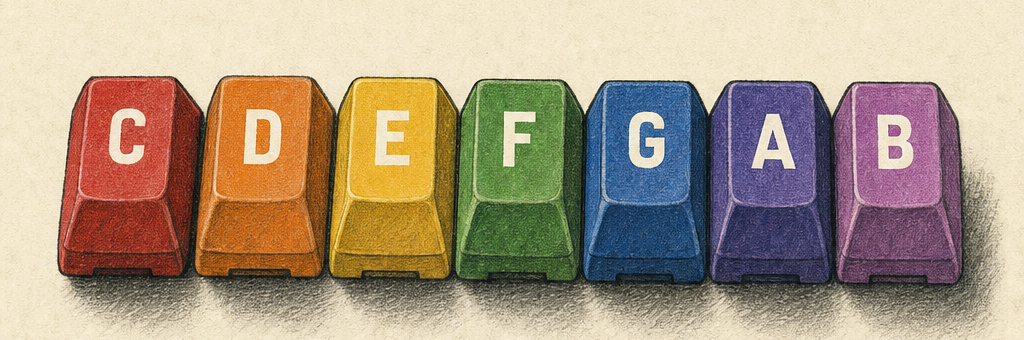
\includegraphics[width=0.62\textwidth]{keys-strip.png}\\[14pt]
\end{center}
{\small\sffamily top line = chord · middle = right hand, one letter per beat, – holds the note · bottom = left hand: bass on 1, then the two-key chord on 2 and 3}\par\vspace{16pt}
\noindent\begin{minipage}[t]{0.23\textwidth}\centering{\chord G}\\[2pt]{\rh l n l}\\[2pt]{\lh g\ \ b+d\ \ b+d}\end{minipage}\hfill\begin{minipage}[t]{0.23\textwidth}\centering{\chord G}\\[2pt]{\rh i – –}\\[2pt]{\lh g\ \ b+d\ \ b+d}\end{minipage}\hfill\begin{minipage}[t]{0.23\textwidth}\centering{\chord C}\\[2pt]{\rh j l j}\\[2pt]{\lh c\ \ e+g\ \ e+g}\end{minipage}\hfill\begin{minipage}[t]{0.23\textwidth}\centering{\chord G}\\[2pt]{\rh i – –}\\[2pt]{\lh g\ \ b+d\ \ b+d}\end{minipage}\par\vspace{14pt}\vspace{2pt}\noindent\begin{minipage}[t]{0.23\textwidth}\centering{\chord D}\\[2pt]{\rh u m u}\\[2pt]{\lh d\ \ w+a\ \ w+a}\end{minipage}\hfill\begin{minipage}[t]{0.23\textwidth}\centering{\chord D}\\[2pt]{\rh i j u}\\[2pt]{\lh d\ \ w+a\ \ w+a}\end{minipage}\hfill\begin{minipage}[t]{0.23\textwidth}\centering{\chord G}\\[2pt]{\rh l – n}\\[2pt]{\lh g\ \ b+d\ \ b+d}\end{minipage}\hfill\begin{minipage}[t]{0.23\textwidth}\centering{\chord D}\\[2pt]{\rh m – –}\\[2pt]{\lh d\ \ w+a\ \ w+a}\end{minipage}\par\vspace{14pt}\noindent\rule{\textwidth}{0.4pt}\par\vspace{12pt}\noindent\begin{minipage}[t]{0.23\textwidth}\centering{\chord Em}\\[2pt]{\rh j l j}\\[2pt]{\lh e\ \ g+b\ \ g+b}\end{minipage}\hfill\begin{minipage}[t]{0.23\textwidth}\centering{\chord Em}\\[2pt]{\rh n – –}\\[2pt]{\lh e\ \ g+b\ \ g+b}\end{minipage}\hfill\begin{minipage}[t]{0.23\textwidth}\centering{\chord C}\\[2pt]{\rh j l m}\\[2pt]{\lh c\ \ e+g\ \ e+g}\end{minipage}\hfill\begin{minipage}[t]{0.23\textwidth}\centering{\chord D}\\[2pt]{\rh u – –}\\[2pt]{\lh d\ \ w+a\ \ w+a}\end{minipage}\par\vspace{14pt}\vspace{2pt}\noindent\begin{minipage}[t]{0.23\textwidth}\centering{\chord G}\\[2pt]{\rh l n l}\\[2pt]{\lh g\ \ b+d\ \ b+d}\end{minipage}\hfill\begin{minipage}[t]{0.23\textwidth}\centering{\chord C}\\[2pt]{\rh l m j}\\[2pt]{\lh c\ \ e+g\ \ e+g}\end{minipage}\hfill\begin{minipage}[t]{0.23\textwidth}\centering{\chord D}\\[2pt]{\rh i j u}\\[2pt]{\lh d\ \ w+a\ \ w+a}\end{minipage}\hfill\begin{minipage}[t]{0.23\textwidth}\centering{\chord G}\\[2pt]{\rh l – –}\\[2pt]{\lh g\ \ b+d\ \ b+d}\end{minipage}\par\vspace{14pt}\vspace{2pt}
\clearpage
\end{document}